\scanpage{135}
% archive sheet number: 134
\figure{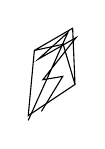
\begin{tikzpicture}[scale=.6]
\draw (0,0)--(.13,1.38)--(.94,1.85)--(.99,.66)--cycle (.13,1.38)--(.74,1.51)--(.99,.66);
\draw (0,-.1)--(.84,1.76)--(.22,1.2)--(1.01,1.65)--(.31,.76)--(.73,.83)--(.28,.09);
\end{tikzpicture}}
\[\left\{\begin{aligned}
&\text{Prismes triangulaires \deleted{\unsure{dans}} pavé + triangles}\\
&\approxeq(\mathrm{Ens})_2\times(\mathrm{Ens})_3\times(\mathrm{Ens})_3
\end{aligned}\right.\]

\noindent\rule{.33\linewidth}{.4pt}
\figure{\begin{tikzpicture}[scale=.75,every node/.style={inner sep=1pt}]
\draw (0,3.95)--(.01,5.45)--(1.53,5.48)--(1.45,3.87)--cycle (.01,5.45)--(.65,6.07)--(2.28,6.07)--(2.11,4.79) (0,3.95)--(.69,4.75)--(1.95,4.73) (1.53,5.48)--(2.28,6.07) (.65,6.07)--(.69,4.75);
\draw (.06,5.3)..controls (2.63,7.33) and (2.16,6.32)..(.32,5.12)..controls (.03,4.73) and (2.62,6.29)..(1.55,5.03)..controls (.59,3.97) and (2.02,3.99)..(1.84,3.99);
\draw (.66,5.11)..controls (1.85,5.37) and (.86,4.47)..(.86,4.09)..controls(.86,3.95) and (1.21,3.94)..(1.34,3.95);
\begin{scope}[xshift=1.13cm,yshift=2.13cm]
\draw (0,0)--(0,1.09)--(1.52,1.17)--(1.55,.05)--cycle (1.55,.05)--(2.96,.03)--(3,1.24)--(1.52,1.17)--(1.81,1.55)--(1.79,2.26)--(2.98,1.25) (0,1.09)--(1.79,2.26)--(.06,.05) (1.79,2.26)--(2.85,.10);
\fill (.83,.55) circle(1.5pt) (2.22,.58) circle(1.5pt);
\draw[->] (-.76,.91)--(3.09,1.99);\draw (-.22,-.3)--(5.81,1.86);
\coordinate (s) at (2.49,0);\node[above left] at (s){$s$};\fill (s) circle(1.7pt);
\draw (s)--(3.39,.59);\node[above right] at (3.39,.59){$u$};
\draw (1.07,-.86)--(3.42,-.85)--(3.47,-1.79)--(1.14,-1.78)--cycle (1.07,-.86)--(s)--(3.42,-.85) (1.14,-1.78)--(s)--(3.39,-1.72) (s)--(2.57,-.60)--(2.22,-1.78) (2.22,-.85)--(2.22,-1.78);
\node[left] at (1.07,-.88){$a'$};\node[right] at (3.42,-.82){$a''$};\node[left] at (2.34,-.65){$a$};\node[right] at (2.57,-.6){$t$};
\node[below left] at (1.14,-1.78){$b'$};\node[below] at (2.22,-1.78){$b$};\node[below right] at (3.42,-1.78){$b''$};
\node at (4.98,.78){$\deleted{\text{bicarré}}$};
\draw (s)--(11.84,2.0);
\draw[thin] (-.91,1.55)..controls (-1.13,.87) and (-.76,-.4)..(-1.39,-.35)..controls(-.92,-.28) and (-1.08,-1.16)..(-.84,-1.88);
\end{scope}
\begin{scope}[xshift=11.24cm,yshift=2.68cm]
\draw (0,0)--(-.03,.93)--(1.42,.98)--(1.48,-.03)--cycle (1.48,-.03)--(2.86,.03)--(2.76,.97)--(1.42,.98);
\draw (0,.95)--(1.6,1.95)--(2.76,.97) (0,.04)--(1.6,1.95)--(1.48,-.03) (0,.04)--(.61,-.95)--(1.48,-.03)--(2.18,-.96)--(2.86,.03) (1.6,1.95)--(2.86,.03) (2.76,.97)--(2.17,-.38) (.61,-.95)--(.82,.42)--(1.63,1.19) (0,.95)--(.62,-.39)--(1.6,1.95);
\draw[line width=1pt] (1.48,-.03)--(1.42,.98)--(1.63,1.19);
\fill (2.09,.43) circle(1.5pt);
\end{scope}
\end{tikzpicture}}

les triangles sur $(a'b')$ et $(a''b'')$ ont $=$ sommet $s$

Si $t$ est le \inserted{$3^e$ sommet du} triangle de base $(a,b)$, le \deleted{\unsure{centre de|cube de}} troisième sommet \inserted{$u$} du triangle de base $(st)$ est le centre du \inserted{\unsure{carr|carré}} $(abb'a')$ et du carré $(abb''a'')$. Donc les deux carré ont $=$ centre\inserted{$u$}, et étant distincts, ne sont pas contenus dans le $=$ pavé -- ils engendrent donc une \unsure{cour.} On peut dire aussi que
\figure{\begin{tikzpicture}[scale=.8]
\fill (-1.4,1.26) circle(3pt);
\draw[gray] (.6,1.62)--(.85,.53)--(1.9,.52)--(2.23,1.51) (3.63,3.88)--(3.66,2.91)--(5.17,2.92)--(5.2,3.91);
\draw (0,0)--(1.57,-.02) (1.72,-.01)--(3.1,-.06)--(3.03,-1)--(3.69,-.65) (0,0)--(0,-.96)--(.44,-.99);
\draw[dashed] (0,-.96)--(1.28,-2.26)--(3.03,-1) (3.68,.03)--(3.69,-.65);
\fill (1.57,-.02) circle(1.8pt) (3.1,-.06) circle(1.7pt) (1.28,-2.26) circle(1.6pt);
\node[above left] at (0,0){$a'$};\node[above] at (1.57,-.02){$\deleted{\unsure{c}}a$};\node[above] at (3.69,.04){$\unsure{a'|a''}$};\node[below left] at (0,-1){$b'$};\node[below] at (3.56,-.73){$b''$};
\end{tikzpicture}}
est un $A_5$ contenu dans un pavé unique, en fait c'est un hexagone \unsure{épointé|épinglé|ponctué} de façon unique en désignant la triade $(d,b',b'')$ -- et il faut choisir un pt $b$ lié aux trois pts de cette triade, i.e. appartenant à la triade \unsure{opposée|apposée}

Card des choix au total $\tfrac12(720\times6\times3)=2^{\unsure{4}}.3^4.5=N:2^3$ -- en effet, la cat. des \deleted{\illegible{1}} graphes cubiques avec bicarré est
\[
\simeq\underbrace{(\mathrm{Ens})_2\times(\mathrm{Ens})_2}_{\text{bicarré}}\times
\underbrace{(\mathrm{Ens})_2}_{\substack{\text{compléter l'enveloppe}\\\text{quasi-trilitaire en}}}
\simeq\operatorname{Tors}((\pm1)^3)
\]
